\documentclass{article}
\usepackage[margin=1in]{geometry}
\usepackage{amsmath, amsthm, amssymb, amsfonts}
\usepackage{graphicx}
\usepackage{xcolor}
\usepackage{enumerate}
\usepackage{environ}
\usepackage{tikz}

\newcommand{\inv}{^{-1}}

\newcounter{pnum}
\NewEnviron{problem}{
    \stepcounter{pnum}
    \begin{center}
        \fbox{
        \begin{minipage}{0.95\linewidth}
            \textbf{\thepnum.} \BODY
        \end{minipage}}
    \end{center}

    \textbf{Solution. }
}

\title{\vspace{-4em}Homework 6 (root finding)}
\author{Hanzhang Yin}
\begin{document}

\maketitle

\begin{problem}
    One view of the secant method: it is a coarser Newton's method. We've seen that it has some of the speed of Newton's method. One might also hope that it enjoys similar convergence properties.\\[-0.5em]
    
    Adapt the convergence proof for Newton's method to show that the secant method also always converges under the following assumptions about the function \(f\) on the interval \([a,b]\):
    \begin{enumerate}[\hspace{2em} i)]
        \item \(f\) is twice continuously differentiable
        \item \(f' > 0\)
        \item \(f''> 0\)
        \item \(f\) has a root \(x\) in the interval
        \item the two initial guesses \(x_0,x_1\) are both to the right of the root.
    \end{enumerate}

    Hint: you will have to use convexity in a slightly more interesting way than in NM -- the graph of \(f\) does not lie above the secant line, but you can argue that the right (well, left!) piece still does.
\end{problem}

\begin{proof}
    The secant method iterates according to the formula:
    \[
        x_{n+1} = x_n - f(x_n) \cdot \frac{x_n - x_{n-1}}{f(x_n) - f(x_{n-1})}.
    \]
    We proceed in steps to show the convergence.
    \\
    \textbf{Monotonicity and Boundedness}
    \\
    \textit{Claim: } The sequence \( \{x_n\} \) is strictly decreasing and bounded below by \( x^\ast \).
    \\
    We will prove the claim by induction
    \begin{itemize}
        \item \textbf{Base Case (\( n = 1 \)):} By assumption, \( x_0 > x^\ast \) and \( x_1 > x^\ast \). WLOG, we can reorder \( x_0 \) and \( x_1 \) such that \( x_0 > x_1 > x^\ast \). Hence, the base case holds.
    
        \item \textbf{Inductive Step:} Assume \( x_{n-2} > x_{n-1} > x^\ast \). We show that \( x_n > x^\ast \) and \( x_n < x_{n-1} \).
    
        From the secant update:
        \[
        x_n = x_{n-1} - f(x_{n-1}) \cdot \frac{x_{n-1} - x_{n-2}}{f(x_{n-1}) - f(x_{n-2})}.
        \]
        \begin{itemize}
            \item Since \( x_{n-2} > x_{n-1} \), we have \( x_{n-1} - x_{n-2} < 0 \).
            \item Since \( f'(x) > 0 \) on \([a, b]\), \( f(x_{n-1}) > f(x_{n-2}) \), so \( f(x_{n-1}) - f(x_{n-2}) > 0 \).
            \item Therefore, the ratio \( \frac{x_{n-1} - x_{n-2}}{f(x_{n-1}) - f(x_{n-2})} < 0 \).
            \item Since \( f(x_{n-1}) > 0 \) (as \( x_{n-1} > x^\ast \ \text{and f is increasing} \)), the term subtracted from \( x_{n-1} \) is positive:
            \[ x_n = x_{n-1} - (\text{Positive Number}) < x_{n-1} \]
            implying \( x_n < x_{n-1} \).
            \item To show \( x_n > x^\ast \), assume \( x_n \leq x^\ast \). Then \( f(x_n) \leq f(x^\ast) = 0 \), contradicting the fact that \( f(x_n) > 0 \) for \( x_n > x^\ast \). Thus, \( x_n > x^\ast \).
        \end{itemize}
    \end{itemize}
    By induction, \( \{x_n\} \) is strictly decreasing and bounded below by \( x^\ast \).
    \\
    \textbf{Convergence of the Sequence}
    \\
    \textit{Claim: } The sequence \( \{x_n\} \) converges to \( x^\ast \).
    \\
    Since \( \{x_n\} \) is strictly decreasing and bounded below by \( x^\ast \), it converges to some limit \( l \geq x^\ast \) by \textbf{MCT}. Suppose, for contradiction, that \( l > x^\ast \).
    
    \begin{itemize}
        \item Since \( f \) is continuous and strictly increasing:
        \[
        \lim_{n \to \infty} f(x_n) = f(l) > f(x^\ast) = 0.
        \]
        \item Consider the secant update:
        \[
        x_{n+1} = x_n - \frac{f(x_n)}{s_n}, \quad \text{where } s_n = \frac{f(x_n) - f(x_{n-1})}{x_n - x_{n-1}}.
        \]
        \item Because \( f \) is convex (\( f'' > 0 \)), the slope \( s_n > f'(x^\ast) > 0 \), so:
        \[
        \left| \frac{f(x_n)}{s_n} \right| < \frac{f(x_n)}{f'(x^\ast)}.
        \]
        \item As \( n \to \infty \), \( f(x_n) \to f(l) > 0 \), meaning the step sizes \( x_n - x_{n+1} \) do not shrink to zero.
        \item This contradicts the convergence \( x_n \to l \), as the step sizes must tend to zero for convergence.
    \end{itemize}
    Thus, \( l = x^\ast \), and the sequence converges to \( x^\ast \).
    \\
    The convexity of \( f \) ensures that the secant line between any two points lies below the graph of \( f \), preventing the iterates \( x_n \) from overshooting the root \( x^\ast \). Thus, \( x_n > x^\ast \) for all \( n \).
    Under the given assumptions:
    \begin{enumerate}
        \item \( \{x_n\} \) is strictly decreasing and bounded below by \( x^\ast \),
        \item By the monotone convergence theorem, \( \{x_n\} \) converges to a limit \( l \geq x^\ast \),
        \item Assuming \( l > x^\ast \) leads to a contradiction, hence \( l = x^\ast \),
        \item Convexity ensures no overshooting, maintaining \( x_n > x^\ast \).
    \end{enumerate}
    \\
    Therefore, the secant method converges to the root \( x^\ast \).
\end{proof}

\newpage

\begin{problem}
    Another view of the secant method, discussed in class, is as a weighted bisection method. Here too, one might hope for a convergence guarantee, because BM is much more robust than NM in that regard.\\[-0.5em]

    Consider a modified secant method which at step \(k\) takes in endpoints \(a_k,b_k\), calculates their weighted midpoint \(c_k\) and then returns two new endpoints \(a_{k+1},b_{k+1}\), one of which is \(c_k\), to which IVT applies. These new endpoints are input to the next step.\\[-0.5em]

    Prove that if \(f\) is continuous on \([a,b] = [a_0,b_0]\) and the IVT applies to \(f\) on the interval, then the sequence \(c_k\) from the modified secant method converges to a root of \(f\).\\[-0.5em]

    Hint: the reason for convergence is \emph{not} the same as for bisection. This would require the stronger assumption that \(f\) is continuously differentiable. In fact:

    [Bonus] Give an example where the sequences \(x_k\) and \(y_k\) converge to different points, so squeeze does not apply.
\end{problem}


\begin{proof}
    Let \( f \) be a continuous function on the interval \( [a_0, b_0] \) such that \( f(a_0) \cdot f(b_0) < 0 \). By the Intermediate Value Theorem (IVT), there exists at least one root \( x \) in \( (a_0, b_0) \) where \( f(x) = 0 \).
    \\
    \textbf{Modified Secant Method Algorithm:}
    \\
    At each iteration \( k \):
    \\
    \begin{enumerate}
        \item \textbf{Compute the Weighted Midpoint by Secant Method:}
        \[
            c_k = \frac{b_k f(a_k) }{f(a_k) - f(b_k)} - \frac{a_k f(b_k)}{f(a_k) - f(b_k)}
        \]
        This point \( c_k \) is the root of the secant line connecting \( (a_k, f(a_k)) \) and \( (b_k, f(b_k)) \) since IVT applies on each intervals within $[a_0, b_0]$.

        \item \textbf{Update the Interval:}
        \begin{itemize}
            \item Determine which subinterval \( [a_k, c_k] \) or \( [c_k, b_k] \) contains a sign change, i.e., where \( f \) changes sign.
            \item Set \( (a_{k+1}, b_{k+1}) \) to be the endpoints of this subinterval.
        \end{itemize}
    \end{enumerate}
    \\
    \textbf{Properties of the Sequences \( \{a_k\} \) and \( \{b_k\} \):}
    \\
    Without loss of generality, assume that \( c_k \) has the same sign as \( a_k \). Then, set \( a_{k+1} = c_k \) and \( b_{k+1} = b_k \) following the bisection method update rule. 
    Consequently, the sequences \( \{a_k\} \) and \( \{b_k\} \) are monotonic, as each endpoint is either updated to a new point within the interval or remains unchanged at each iteration.
    Formally speaking: 
    \begin{itemize}
        \item \textbf{Monotonicity:}
        \begin{itemize}
            \item \( \{a_k\} \) is non-decreasing.
            \item \( \{b_k\} \) is non-increasing.
        \end{itemize}
        \item \textbf{Boundedness:}
        \begin{itemize}
            \item \( \{a_k\} \subseteq [a_0, b_0] \).
            \item \( \{b_k\} \subseteq [a_0, b_0] \).
        \end{itemize}
        \item \textbf{Convergence:}
        \begin{itemize}
            \item Both sequences converge due to monotonicity and boundedness by \textbf{MCT}:
            \[
                \lim_{k \to \infty} a_k = a, \quad \lim_{k \to \infty} b_k = b, \quad \text{with} \quad a \leq b.
            \]
        \end{itemize}
    \end{itemize}
    \\
    The next step that we want to do is to argue that at least one of the element $a$ or $b$ converges to zero.
    \\
    \textbf{Case 1:} \( a = b \)
    \\
    The interval \( [a_k, b_k] \) shrinks to the point \( a = b = x \).
    Since \( f(a_k) \cdot f(b_k) < 0 \) for all \( k \), and \( f \) is continuous, we have:
    \[
        \lim_{k \to \infty} f(a_k) = f(a), \quad \lim_{k \to \infty} f(b_k) = f(b).
    \]
    It must be that \( f(a) = 0 \), because otherwise \( f(a) \) and \( f(b) \) would have the same sign, contradicting \( f(a_k) \cdot f(b_k) < 0 \).
    Therefore, \( c_k \in [a_k, b_k] \) converges to \( x = a = b \), which is a root of \( f \).
    \\
    \textbf{Case 2:} \( a < b \)
    \\
    The interval \( [a_k, b_k] \) in this case does not shrink to a point.
    \\
    Suppose for contradiction that neither $a$ and $b$ is a root of the function $f$. Then pick an arbitrary number $k$ s.t. it is big enough that $a_k$ and $b_k$ 
    are close to the $a_{\infty}$ and $b_{\infty}$. 
    Since $a$ and $b$ are not roots, $f(a_k), f(b_k) \neq 0$ so that IVT can be applied.
    From IVT, we can find a point $c_k$ s.t. $c_k \in [a_k, b_k]$ (i.e. $a_k < c_k < b_k$). 
    From our assumption above, noting that $(a_k)$ and $(b_k)$ are monotonic sequence s.t. for every $k$, $a_k \leq b_k$. Also noticing that in this case, we assume $a < b$.
    Hence, we can draw a conclusion that:
    \[ a_k \approx a < b = b_k, \text{when k} \to \infty \]
    Since $c_k$ as the new midpoint is within $[a_n, b_n]$, apprximately $a \leq c_n \leq b$. Also, base on our bisection method update rule $c_n$ is the next term of the sequence $\{a_{k}\}$ or $\{b_{k+1}\}$.
    \\
    At this stage, WLOG, we can assume that $c_k$ to be the next further term of sequence $\{a_{k}\}$, then $a_{k + 1} > \lim_{k \to \infty} a_k = a$, we derived a contradiction.
    \\
    \textbf{*Case 3:} 
    \\
    Since \textit{case 2} is not sound, suppose \textit{case 1} is not the case, then surely one of $a$ and $b$ converges to the root (denote it as $x$).
    Lets assume $a = x$, WLOG, then, for $k \to \infty$, $f(a_k) \approx 0$. Then then next point of $c_k$, which is $c_{k + 1}$ can be represented as:
    \[ c_{k} = \frac{b_k f(a_k) }{f(a_k) - f(b_k)} - \frac{a_k f(b_k)}{f(a_k) - f(b_k)} = \frac{0}{0 - f(b_k)} - \frac{f(b_k)}{0 - f(b_k)} a_k \approx a_k \]
    Then the ``next term'' is approximately $a_k$. By knowing that,
    \[ c_k = a_{k + 1} \ or \ c_k = b_{k+1} \]
    But we know from our assumption that,
    \[ c_k \approx a_{k + 1} < a < b < b_{k + 1} \]
    so $c_k \neq b_{k+1}$. Then applying limit on both side for equation $c_k = a_{k + 1}$, then:
    \[ \lim_{k \to \infty} c_k = \lim_{k \to \infty} a_{k + 1} \Rightarrow c = a \]
    By continuously updating the midpoint, root $x = a$ ultimately.
\end{proof}

\begin{problem}
    Suppose \(f(x)\) and \(g(x)\) are functions with a common root \(x=a\).
    \begin{enumerate}[\hspace{2em}a)]
        \item Prove that a solution to the homotopy continuation initial value problem
    \[x'(t) = -\frac{H_t}{H_x}\ \ \ \ x(0) = a\]
    is the constant function \(x=a\).
        \item Give an example where the solution above is \emph{not} unique.
    \end{enumerate}

    Hint: see handout for a picture of (a). Think about how it could be adapted (b); you can even use the tool to help you construct an example.
\end{problem}

\begin{proof}
    \textbf{Part (a): Proving \( x(t) = a \) is a Solution}
    \\
    Let us define the homotopy \( H(x, t) \) as
    \[
        H(x, t) = (1 - t) f(x) + t g(x).
    \]
    Since \( f(a) = g(a) = 0 \), it follows that \( H(a, t) = 0 \) for all \( t \in [0, 1] \).
    \\
    We need to show that \( x(t) = a \) satisfies the differential equation
    \[
        x'(t) = -\frac{H_t}{H_x}, \quad x(0) = a.
    \]
    \textit{Computing the Partial Derivatives:}
    \\
    First, compute \( H_t \) and \( H_x \):
    \[
        H_t(x, t) = -f(x) + g(x),
    \]
    \[
        H_x(x, t) = (1 - t) f'(x) + t g'(x).
    \]
    Evaluate these at \( x = a \):
    \[
        H_t(a, t) = -f(a) + g(a) = -0 + 0 = 0.
    \]
    \[
        H_x(a, t) = (1 - t) f'(a) + t g'(a).
    \]
    Note that \( H_x(a, t) \) may not be zero unless both \( f'(a) \) and \( g'(a) \) are zero.
    \\
    \textit{Computing \( x'(t) \) at \( x = a \):}
    \\
    Substitute \( x(t) = a \) into the differential equation:
    \[
        x'(t) = -\frac{H_t(a, t)}{H_x(a, t)} = -\frac{0}{H_x(a, t)} = 0.
    \]
    Therefore,
    \[
        x'(t) = 0, \quad x(0) = a.
    \]
    This implies that \( x(t) = a \) for all \( t \in [0, 1] \).
    \\
    \textbf{Conclusion:}
    \\
    The constant function \( x(t) = a \) is a solution to the homotopy continuation initial value problem.
\end{proof}

\begin{proof}
    \textbf{Part (b): Example Where the Solution is Not Unique}
    \\
    We will construct specific functions \( f(x) \) and \( g(x) \) with a common root at \( x = a \) such that the initial value problem
    \[
        x'(t) = -\frac{H_t}{H_x}, \quad x(0) = a,
    \]
    has multiple solutions.
    \\
    \textbf{Example Functions:}
    \\
    Let
    \[
        f(x) = (x - a)^{1/3}, \quad g(x) = -(x - a)^{1/3}.
    \]
    Both functions have a root at \( x = a \):
    \[
        f(a) = g(a) = 0.
    \]
    \textbf{Constructing the Homotopy:}
    \\
    Define
    \[
        H(x, t) = (1 - t) f(x) + t g(x) = (1 - t)(x - a)^{1/3} + t ( - (x - a)^{1/3} ) = (1 - 2t)(x - a)^{1/3}.
    \]
    Compute \( H_t \) and \( H_x \):
    \[
        H_t(x, t) = -f(x) + g(x) = - (x - a)^{1/3} - (x - a)^{1/3} = -2 (x - a)^{1/3},
    \]
    \[
        H_x(x, t) = (1 - 2t) \cdot \frac{1}{3} (x - a)^{-2/3}.
    \]

    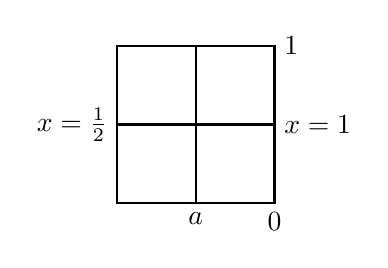
\begin{tikzpicture}
        \begin{scope}[xshift=6cm] % Shift this graph horizontally
            % Box and divisions
            \draw[thick] (0,0) rectangle (2,2);
            \draw[thick] (1,0) -- (1,2); % Vertical line
            \draw[thick] (0,1) -- (2,1); % Horizontal line
        
            % Labels
            \node[below] at (2,0) {0};
            \node[left] at (0,1) {\(x= \frac{1}{2}\)};
            \node[right] at (2,2) {1};
            \node[right] at (2,1) {\(x=1\)};
            \node[below] at (1,0) {\(a\)};
        \end{scope}
    \end{tikzpicture}
    \\
    When $t$ shifts from $0 \to 1$, at a certain point for $t$ the homotopy will coincide with the x-axis completely. 
    This leads a shift from the solution $x=a$ when $t=0$ to the solution $x$ equals to every possible points on the x-axis between $x = \frac{1}{2}$ to $x = 1$.
    This clearly makes the solution \textbf{NOT Unique} during the approximation.
\end{proof}

\end{document}
